% 四阶龙格库塔法
% 龙格库塔|常微分方程|ode|数值计算

\pentry{中点法解常微分方程(组)\upref{OdeMid}}

\textbf{龙格库塔法}是一类数值解微分方程的算法, 其中较常见的是\textbf{四阶龙格库塔法}. 这里不进行推导, 仅仅给出公式如下($y_n, t_n, h$ 的定义类比\autoref{OdeNum_eq5}~\upref{OdeNum})
\begin{equation}\label{OdeRK4_eq1}
y_{n+1} = y_n + \frac h6 (k_1 + 2k_2 + 2k_3 + k_4)
\end{equation}
其中
\begin{equation}\label{OdeRK4_eq2}
\ali{
k_1 &= f(y_n, t_n) 
& k_2 &= f \qty(y_n + h\frac{k_1}{2}, t_n + \frac h2 )\\
k_3 &= f \qty( y_n + h\frac{k_2}{2}, t_n + \frac h2 ) \qquad
&k_4 &= f(y_n + hk_3, t_n + h)
}\end{equation}
由以上两式, 不难把该算法拓展到方程组的情况. 对于 $N$ 元微分方程组
\begin{equation}
\begin{cases}
y'_1(t) = f_1(y_1,\dots, y_N, t)\\
y'_2(t) = f_2(y_1,\dots, y_N, t)\\
\qquad\;\; \vdots\\
y'_N(t) = f_N(y_1,\dots, y_N, t)
\end{cases}
\end{equation}
我们可以把该式记为矢量函数的形式
\begin{equation}\label{OdeRK4_eq4}
\bvec y'(t) = \bvec f(\bvec y, t)
\end{equation}
现在我们仅需要把\autoref{OdeRK4_eq1} 和 \autoref{OdeRK4_eq2} 中的所有 $y_i$ 和 $k_i$ 都变为 $N$ 维列矢量 $\bvec y_i$ 和 $\bvec k_i$ 即可将微分方程拓展为微分方程组.

\subsection{例程}

到目前为止, 我们每求一个微分方程的数值解都要重新写一次程序, 对于一些较为复杂的算法这样做效率较低. 我们这里不妨把四阶龙格库塔法写到一个单独的函数文件 odeRK4.m 中, 当我们要解某个特定的方程时, 只需把\autoref{OdeRK4_eq2} 中的 $f(y, t)$ 作为自变量输入即可解出 $y(t)$.

\begin{lstlisting}[language=matlab, caption=odeRK4.m]
function [Y, t] = odeRK4(f, tspan, Y0, Nt)
Nvar = numel(Y0);  % 因变量的个数
dt = (tspan(2) - tspan(1)) / (Nt-1); % 计算步长
Y = zeros(Nvar, Nt); % 预赋值
Y(:, 1) = Y0(:); % 初值
t = linspace(tspan(1), tspan(2), Nt);

for ii=1:Nt-1
    K1 = f(Y(:,ii)          , t(ii)      );
    K2 = f(Y(:,ii)+K1*dt/2  , t(ii)+dt/2 );
    K3 = f(Y(:,ii)+K2*dt/2  , t(ii)+dt/2 );
    K4 = f(Y(:,ii)+K3*dt    , t(ii)+dt   );
    Y(:,ii+1) = Y(:,ii) + dt/6 * (K1+2*K2+2*K3+K4);
end
end
\end{lstlisting}

我们先来看第 1 行的函数声明, 输入变量中,\verb|f| 是\autoref{OdeRK4_eq4} 中 $\bvec f(\bvec y, t)$ 的函数句柄\upref{MatFun}, \verb|tspan| 是一个 \verb|2×1| 的列矢量, \verb|tspan(1)| 是初始时间, \verb|tspan(2)| 是终止时间, \verb|Y0| 是一个列矢量, \verb|Y0(ii)| 是第 \verb|ii| 个因变量的初始值, \verb|Nt| 是 $t_n$ 的个数, \verb|tspan| 定义的时间区间被等分为 \verb|Nt - 1| 个小区间. 因变量中, \verb|Y| 的行数是因变量的个数, 列数是 \verb|Nt|, \verb|t| 是一个行矢量, 由第 6 行定义, \verb|Y(ii, jj)| 就是第 \verb|ii| 个变量在 \verb|t(jj)| 时刻的值. 第 5 行把初值 \verb|Y0| 赋给 \verb|Y| 的第 1 列, 第 8-14 行的循环根据\autoref{OdeRK4_eq1} 和\autoref{OdeRK4_eq2} 的矢量形式由 \verb|Y| 的第 \verb|ii| 列($\bvec y_i$)求第 \verb|ii+1| 列($\bvec y_{i+1}$).

我们先来用这个函数来计算“天体运动的简单数值计算\upref{KPNum0}” 中的问题. 我们令因变量 $\bvec y$ 的四个分量依次为一阶方程组(\autoref{OdeNum_eq4}~\upref{OdeNum})
\begin{equation}\label{OdeRK4_eq5}
\begin{cases}
x' = v_x\\
y' = v_y\\
v'_x = -GMx/(x^2 + y^2)^{3/2}\\
v'_y = -GMy/(x^2 + y^2)^{3/2}
\end{cases}
\end{equation}
中的 $x, y, v_x, v_y$. 程序代码如下

\begin{lstlisting}[language=matlab, caption=keplerRK4.m]
function keplerRK4
% 参数设定
GM = 1; % 万有引力常数乘以中心天体质量
x0 = 1; y0 = 0; % 初始位置
vx0 = 0; vy0 = 0.7; % 初始速度
tspan = [0; 4]; % 总时间和步数
Nt = 100; % 步数

Y0 = [x0; y0; vx0; vy0]; % 因变量初值
f = @(Y, t)fun(Y, t, GM);
[Y,~] = odeRK4(f, tspan, Y0, Nt);

% 画图
figure; hold on;
plot(Y(1,:), Y(2,:));
scatter(0, 0);
axis equal;
end

function Y1 = fun(Y, ~, GM)
% 因变量
x = Y(1); y = Y(2);
vx = Y(3); vy = Y(4);
Y1 = zeros(4,1); % 预赋值
Y1(1) = vx;
Y1(2) = vy;
temp = -GM /(x^2 + y^2)^(3/2);
Y1(3) = temp * x;
Y1(4) = temp * y;
end
\end{lstlisting}

运行结果如\autoref{OdeRK4_fig1} 所示.

\begin{figure}[ht]
\centering
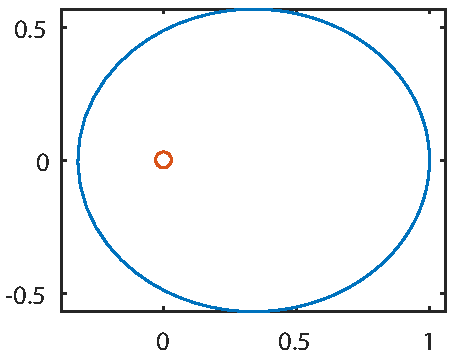
\includegraphics[width=7cm]{./figures/OdeRK4_1.pdf}
\caption{运行结果} \label{OdeRK4_fig1}
\end{figure}

我们先来看函数 \verb|fun| (20 行), 这个函数就相当于\autoref{OdeRK4_eq5}. 第一个输入变量 \verb|Y| 是一个列矢量, 是 $\bvec y_n$ 的值, 第二个输入变量是 $t$, 但由于\autoref{OdeRK4_eq5} 中没有出现 $t$, 我们用波浪线代替. 第三个输入变量是参数 $GM$, 即万有引力常数和中心天体质量之积. 输出变量 \verb|Y1| 是一个列矢量, 是 $\bvec y'_n$ 的值.

再来看主函数 \verb|KeplerRK4| (第 1 行), 参数设定中除了步数从 4000 变为了 100, 其他都和“天体运动的简单数值计算\upref{KPNum0}” 中的程序一样, 然而这里运行结果却精确得多(曲线几乎闭合), 可见这种算法的优越性.

主函数第 10 行中将 \verb|fun(Y, t, GM)| 变为函数句柄 \verb|f(Y, t)|, 这样 \verb|GM| 就可以在“参数设定” 中设置, 而不用在 \verb|fun| 函数内部设置. 第 11 行调用了上文中的 \verb|odeRK4| 函数解方程组, 由于我们在画图时不需要用 \verb|t|, 所以把第二个输出变量改为波浪线.
